\documentclass[a4paper]{article}
\input{/home/luca/Dotfiles/config/nvim/tex/preamble.tex}
%Architectures and systems for biological data processing
\title{Random Walk with Restart (RWR) on Biological Graphs for GPUs}

\begin{document}
\maketitle
\tableofcontents
\newpage

\section{Introduction to the problem}

Many problems in biomedicine can be defined as a ranking problem, given
a set of candidate components, they are ranked relatively based on a 
set of known components. One example is the identification of cellular components 
(genes, proteins, microRNA or other molecules) that are associated with a given disease.
Since the relations between known and candidate components can be naturaly represented as 
a graph, many network-based algorithm has been proposed. Among those, random walk
with restart (RWR) has shown to be the state-of-the-art for those problems.\\
From an abstract perpsective RWR can be seen as multiple random walkers, each one
positioned in one known component, travelling randomly through the graph but with
the addition that at each itration $t$ they have a probability of 
returning directly to the initial node.

Random walk with restart can be computed iteratively according to the 
following function
\begin{equation}
    P_{t} = (1-r)W'P_{t-1} + rP_0
\end{equation}
$P_0$ is the restart vector that represents the initial value of $P$ (e.g.
intial expression levels of a genes). $r$ is the
probability of the random walker to restart at initial position. $W$ is the
adjacency matrix of the graph $G=(E,V)$ which represents the relations between
cellular components, this binary matrix $W$ is than converted into $W'=WD^{-1}$,
where $D$ is the degree vector, which represents the probability of the 
random walker to go from node $u$ to all its neighbors.\\
The specific value of $r$ has little effect on the results of network
propagation over a sizable range, in our case it is setted to 0.6.\\
At each time point $t$, the random walk either flows from the current node $u$
to a randomly chosen neighbour $v \in V$ or restarts at one gene in $P_0$.\\
The propagation of $P_t$ strictly depends on $P_{t-1}$ and is run iteratively
with sufficient step until $P_{t}$ converges to a steady-state $P$.\\
Here the algorithm do not check if $P_{t} = P_{t-1}$ but it is repeated a fixed
number of times.

\section{Sequential algorithm}

The first sequential algorithm considered performs the RWR computing iteratively
formula $(1)$ for a fixed number of steps. The sum and multiplication of the
matrices are done using the library Eigen, which is a high-level C++ library for linear
algebra. This runs way faster than computing all these algebric computation
using nested for loop.\\
Since one of the major problem of performing the RWR using the matrix multiplication is the
size of the matrix $W$ another sequential was build which performs propagation
using the CSR representation of the matrix $W$.\\
Since the second sequential algorithm is faster than the first, every speedup
is considered with respect to the propagation using CSR.\\
Below it is briefly explained the concept behind the CSR propagation since it is 
fairly similar to the parallel algorithm.
\newpage
Each iteration $t$ can be viewed in two parts.
\begin{enumerate}
    \item Multiplication of the $W'P_{t-1}$
    \item Multiply the $1-r$ and sum with $rP_0$
\end{enumerate}
At each time we need to store $P_t, P_{t-1}$ and $P_0$ which for convenience is
directly stored as $rP_0$.
Using a CSR representation of the graph the algorithm is the following:
\begin{enumerate}
    \item $rP_0$ is computed once at the begining of the algorithm
    \begin{figure}[H]
        \centering
        \incfig{propot1}
        \label{fig:propot1}
    \end{figure}
    \item The value $P_{t-1}[i,j]$, which represents the propagation value in
        node $i$ of patient $j$, is propagated in the following way
        \[
            P_t[k,j] = P_t[k,j] + P_{t-1}[i,j]/D[i]
        \] 
        Where $k \in$ Neighbours($i$) and $D$ is the degree of node $i$.\\
        Then $P_{t}[i,j] =  P_{t}[i,j] - P_{t-1}[i,j]$.\\
        Using the analogy with the random walker: the more neighbours a node
        has, the less is the probability of walking to that neighbour.\\
        The second part is instead given by the fact that the random walker
        cannot remain in its node.
    \begin{figure}[H]
        \centering
        \incfig{propot2}
        \label{fig:propot2}
    \end{figure}
    \item When all nodes have propagated they are multiplied by $1-r$ which is
        the probability of not restarting to the intial condition and then
        summed with $rP_0[i,j]$.
    \begin{figure}[H]
        \centering
        \incfig{propot3}
        \label{fig:propot3}
    \end{figure}
\end{enumerate}

\newpage
\section{Parallelization in cuda}
The following three groups of kernels (1,3,5) represents the progression to the final
speedup, which is achieved through kernel 3  + kernel 5.\\
Kernel 1 is the first attempt to parallelization, using a similar algorithm
of the sequential.
It uses a frontier that represents all the nodes different from 0 at
time $t$ but has many atomic operations which are necessary for the
result.\\
Kernel 3 reduced the number of atomic operations and uses virtual warp, this
improves the perfomance but still lack the use of shared memory for reason that
I am going to explain below.\\
Kernel 5 use the shared memory performing the propagation of a single patient on a 
single block in sequential, this is faster but can be done only for small
graph (in my case less than 2000).\\
The final parallelization is done by employing kernel 5 when the number of nodes
fit into the shared memory and in all other cases Kernel 3.

\subsection{Kernel 1}
The first attempt to parallelization is similar to the sequential descripted above.\\
It contains 3 kernels, each one representing one of the steps that were
mentioned in the CSR sequential.
\begin{enumerate}
    \item \textbf{InitKernel}\\
        This kernel creates in parallel, for a given patient, the $rP_0$.
        If the initial value is different from 0, it sets a flag for node $i$ to 1.\\
        This flag is than used to create the frontier nodes that needs to be
        propagated.
    \item \textbf{PropagationKernel} \\
        This is the kernel that performs the propagation of the nodes.\\
        Since each node needs to update its neighbours and also other nodes
        maybe updating the same neighbour the sum must be done using
        \code{atomicAdd}.\\
        In order to check if a node was already in the frontier or it is
        new the control over the \code{flag} is atomic (\code{atomicCAS})
        and also the counter of nodes in the frontier is atomic.\\
        All of these needed atomic operations slow down the process.
    \item \textbf{RestartKernel} \\
        The multiplication of $(1-r)$ and then sum $rP_0$ is performed in a
        separate kernel since we need to be sure that all nodes have propagated.
\end{enumerate}

\subsection{Kernel 3}
This is the final kernel which is used to execute the RWR.\\
It is divided into two kernels and it does not use a frontier.\\
The idea behind this kernel is that instead of propagating each node to its own
neighbours, each node query the neighbours and update itself, in this way all
this atomic add operations on its neighbours becomes only a memory access.\\
At each time all the nodes are updated with their neighourbs, this could waste
some time in the first iterations but it was assumed the following:
\begin{enumerate}
    \item Nodes propagated quickly even starting with the matrix full at 10\%
        wasting only the first few iterations.
    \item When we perform propagation on a gene expression matrix many genes
        have an expression different from zero.
\end{enumerate}

The first kernel compute $rP_0$ as before without computing any frontier.\\
The second kernel instead propagates each node using only one
\code{atomicAdd}.\\
This kernel also use the concept of \textbf{virtual warp} which means that each Warp is 
divided by \code{VWARP\_SZ} in order to better deal with the diversity in the
degrees of the graph and coalescing memory access of the \code{VWARP\_SZ}
consecutive edges.\\
This kernel do not exploit shared memory since I was not able to tile in anyway
the graph, e.g. if my shared memory length is 1024, nothing prevents the node
$11$ to have as neighbour the node 1025.\\
For this reason kernel 5 was developed, which exploit shared memory, but it can be 
used only when there is a small number of nodes.

\subsection{Kernel 5}
Since we cannot have only part of $P_t$ and $P_{t-1}$ in the shared memory, this
kernel store them entirely but can be used only when the size of the shared memory of 
the block is less than the size of nodes.\\
E.g. with my GeForce GTX 1050 Ti the maximum number of nodes is near 2000.\\
The idea of this kernel is that each block performs in sequential only one
patient.\\
Sequential in this case means that each block performs in parallel a
portion of the propagated vector of a single patient, using virtual warp,
and then proceed to the rest of the vector.\\
Here we do not get rid of the \code{atomicAdd} but in newer graphic card
\code{atomicAdd} on the shared memory performs faster than in global memory.

\newpage
\section{Testing}
Tests have been performed using random graphs and biological graphs on a GPU
GeForce GTX 1050 Ti and CPU Intel(R) Core(TM) i7-8750H CPU @ 2.20GHz.

\subsection{Random graph}

The first tests are done using random graphs and random mutation matrix (binary
matrix).\\
The edge list is randomly generated starting from a number of nodes and the
density of the graph (or the average number of degrees) using the Erdős-Rényi
algorithm.\\
The mutation matrix are generated given a number of patients and the density
of the matrix.

\subsubsection{Kernel 1 Vs Sequential}

The following histogram show the speedup of the Kernel 1 with respect to the
sequsequential.\\
Each propagation is characterized
\begin{itemize}
    \item Number of nodes (1000, 2000, 5000, 10000)
    \item Density of the graph (0.2, 0.5, 0.8)
    \item Density of the mutation matrix (0.1, 0.5, 0.8)
\end{itemize}

\begin{figure}[H]
    \centering
    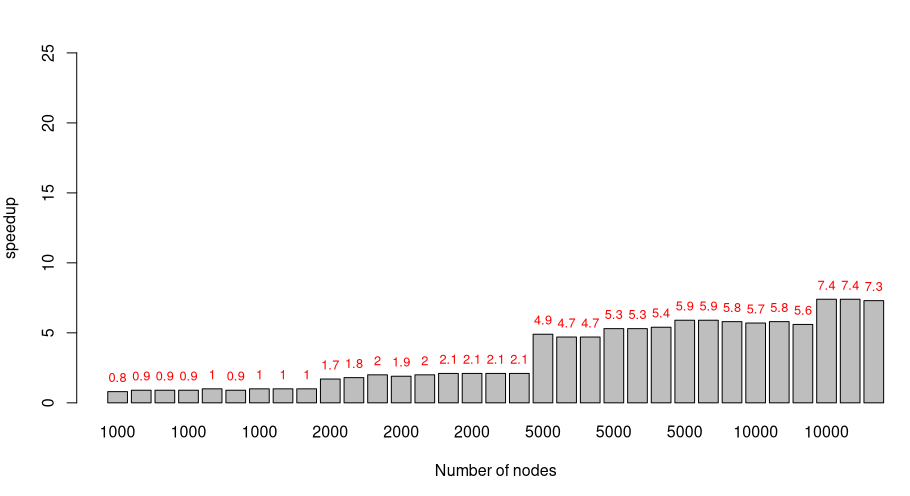
\includegraphics[width=\textwidth]{img/2020-07-12-20:50:02.png}
\end{figure}

The most influential parameters is the number of nodes. 
Even if Kernel 1 depends on the mutation matrix density, given a graph with 20\%
of edges present, the frontier tend to fill up quickly.

\newpage
\subsubsection{Kernel 3 + 5 Vs Sequential}

\begin{figure}[H]
    \centering
    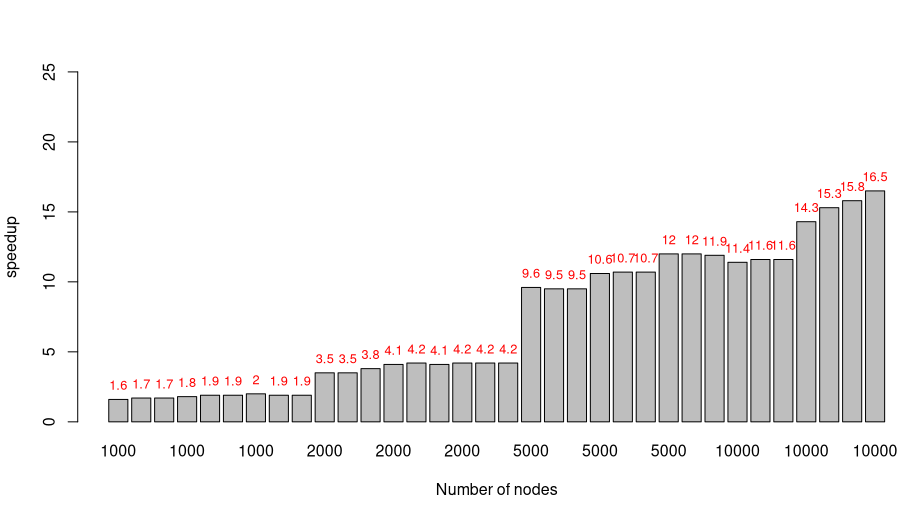
\includegraphics[width=\textwidth]{img/2020-07-12-20:56:05.png}
\end{figure}
Here we can see that increasing the density of the graph we also have a
speedup.\\
This is beacuse the input depends not only on the number of nodes but also on
the number of edges, e.g. when number of nodes equals 5000 and the density of the graph is 0.1 there are
roughly $3*10^6$ edges, instead with a density of 0.8 there are $5*10^6$
edges.\\
The speedup of Kernel 3 with respect to Kernel 1 is in general 2x.

Since we can use the Kernel 5 up to a certain number of nodes here is the final
speedup on random graph given by Kernel 3 + Kernel 5.

\begin{figure}[H]
    \centering
    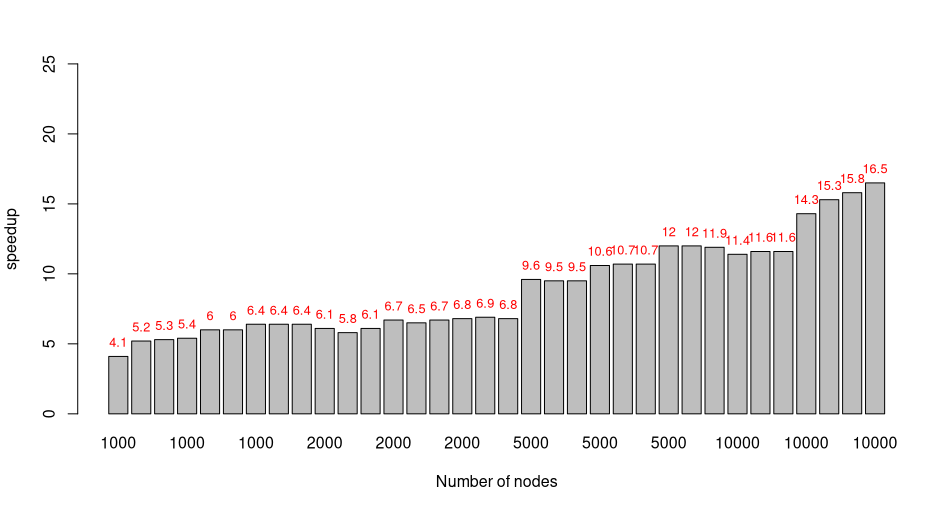
\includegraphics[width=\textwidth]{img/2020-07-12-21:07:10.png}
\end{figure}


\newpage
\subsection{Biological graph}
The speedup in the biological graph is not as high as the speedup of the random
graphs.\\
This is mainly due to the fact that biological graphs are way more sparse and do
not follow any specific distribution, while the degrees of the random graphs
presented above generally follows a gaussian distribution.

\begin{figure}[H]
    \centering
    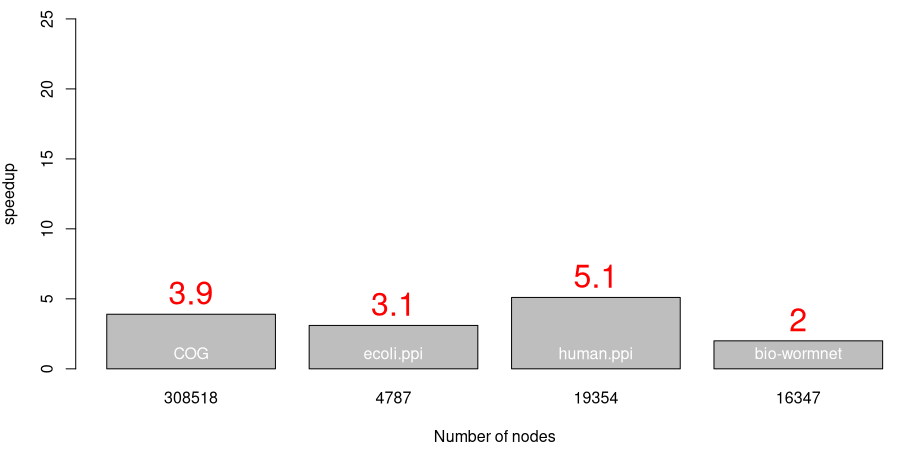
\includegraphics[width=\textwidth]{img/2020-07-13-00:54:48.png}
\end{figure}

In order to test the hypothesis of the gaussian distribution I have constructed
for each biological graph a corresponding synthetic graph with the algorithm
used for random graphs.
\begin{figure}[H]
    \centering
    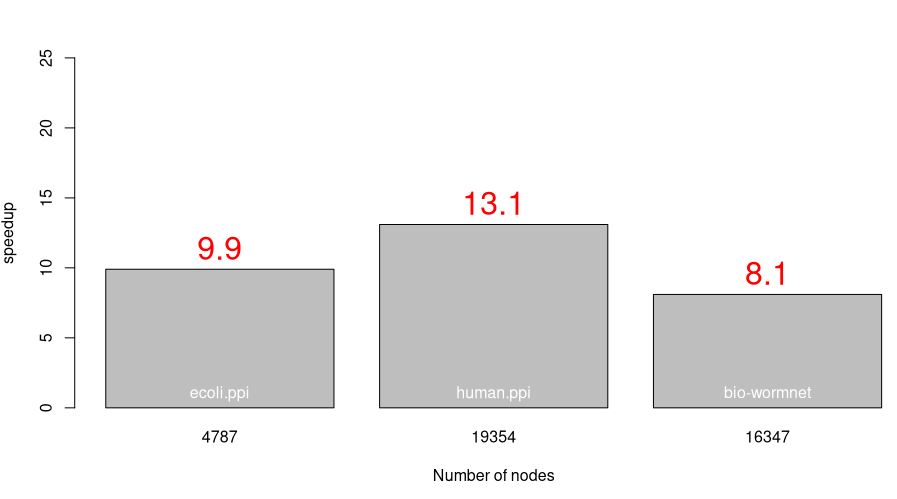
\includegraphics[width=\textwidth]{img/2020-07-13-01:51:52.png}
\end{figure}

Also using the profiler \code{nvvp} I have checked the \textbf{warp execution
efficiency of the kernel} in both the biological and the artificialy biological
graphs and they are respectively 44\% and 81\%.


\section{Conclusion}
The presented parallelization of RWR can reach up to 16.5x of
speedup for graphs that follows a gaussian distribution 
but is not able to reach those speedup for biological graphs, having a peak of
5x.\\
On the other hand this approach is able to perform RWR parallel using the CSR
representation of the graph while most of the RWR implementations need to load
the whole adjacency matrix.


\end{document}
